\documentclass[12pt,a4paper,oneside]{book}

%%%%%%%%%%%%%%%%%%%%%%%%%%%%%%%%%%%%%%%%%%%%%%%%%%%%%%%%%%%%%%%%%%%%%%%%%%%%%%%
% start of the preamble
%%%%%%%%%%%%%%%%%%%%%%%%%%%%%%%%%%%%%%%%%%%%%%%%%%%%%%%%%%%%%%%%%%%%%%%%%%%%%%%

% set the margins to 1 inch
\usepackage[margin=1in]{geometry}
% for including figures
\usepackage{graphicx}
% use etoolbox package for patching \chapter command to get no page numbering
% in the front matter
\usepackage{etoolbox}
% for equation formatting
\usepackage{amsmath,amsthm}
% bibliography packages (square brackets, numbers, and other options etc.)
\usepackage[square,numbers,sort&compress,comma,sectionbib]{natbib}
% set the spacing between bibliography entries
\setlength{\bibsep}{12pt}
% for having separate bibliographies for each chapter
% \usepackage{chapterbib}
% sets default double spacing and for use of the
% \doublespacing and \singlespacing commands
\usepackage[doublespacing]{setspace}
% for getting rid of over/under-full hbox warnings
\usepackage[T1]{fontenc}
% for doing custom 'description' lists used to create the ListOfPublishedPapers
\usepackage{enumitem}
% for doing custom 'description' lists used to create the ListOfPublishedPapers
\usepackage{calc}
% for getting correct word breakup when hyphenating
\hyphenation{con-sti-tu-tion-al}

%%%%%%%%%%%%%%%%%%%%%%%%%%%%%%%%%%%%%%%%%%%%%%%%%%%%%%%%%%%%%%%%%%%%%%%%%%%%%%%
% adjust the table of contents to have 12 pt font and same font family as the
% rest of the document
%%%%%%%%%%%%%%%%%%%%%%%%%%%%%%%%%%%%%%%%%%%%%%%%%%%%%%%%%%%%%%%%%%%%%%%%%%%%%%%

% package for using \cft* commands used below
\usepackage{tocloft}

% change font for chapters, sections, subsections, and subsubsections entries
% in the table of contents
\renewcommand{\cftchapfont}{\normalfont\rmfamily\bfseries}
\renewcommand{\cftsecfont}{\normalfont\rmfamily}
\renewcommand{\cftsubsecfont}{\normalfont\rmfamily}
\renewcommand{\cftsubsubsecfont}{\normalfont\rmfamily}

% no page numbers for table of contents
\tocloftpagestyle{empty}

% remove white space above table of contents heading and below it.
\setlength{\cftbeforetoctitleskip}{-27.73pt}
\setlength{\cftaftertoctitleskip}{0pt}

% change font for the table of contents heading
\renewcommand{\cfttoctitlefont}{\normalfont\rmfamily\bfseries}

%%%%%%%%%%%%%%%%%%%%%%%%%%%%%%%%%%%%%%%%%%%%%%%%%%%%%%%%%%%%%%%%%%%%%%%%%%%%%%%
% Customize Headings for Chapters and sections to all be same font, size, and
% minimize white space
%%%%%%%%%%%%%%%%%%%%%%%%%%%%%%%%%%%%%%%%%%%%%%%%%%%%%%%%%%%%%%%%%%%%%%%%%%%%%%%

% for using \titleformat and \titlespacing commands below
\usepackage[explicit]{titlesec}

% format chapter headings using the following two commmands:
%
% \titleformat{<command to format>}[<shape>]{<format>}{<label format>}{<label spacing>}{<before title code>}
%
% \titlespacing{<command>}{<distance from left margin>}{<before verticle space>}{<after verticle space>}
%

% format chapter headings
\titleformat{\chapter}[display]{\normalfont\bfseries}
{\chaptertitlename\ \thechapter}{0pt} {#1}
\titlespacing{\chapter}{0pt}{-27.73pt}{2em}

% format section headings
\titleformat{\section}[block]{\normalfont\bfseries} {\thesection}{0.5em} {#1}
\titlespacing{\section}{0pt}{\parskip}{\parskip}

% format subsection headings
\titleformat{\subsection}[block]{\normalfont\bfseries}
{\thesubsection}{0.5em} {#1}
\titlespacing{\subsection}{0pt}{\parskip}{\parskip}

% format subsubsection headings
\titleformat{\subsubsection}[block]{\normalfont\bfseries}
{\thesubsubsection}{0.5em} {#1}
\titlespacing{\subsubsection}{0pt}{\parskip}{\parskip}

% if you are going to use other headings they will also have to be formated
% using the \titleformat and \titlespacing commands

% format \section* headings so there is a one line space after them and they
% are added to the table of contents. Only the bibliographies are \section* and
% must be added to the bibliography. For some reason the bibliography headings
% do not have a space after the them without this modification
\titleformat{name=\section,numberless}[block]{\normalfont\bfseries}
{}{0pt}{\addcontentsline{toc}{section}{#1}#1}
\titlespacing{name=\section,numberless}{0pt}{\parskip}{12pt}

%%%%%%%%%%%%%%%%%%%%%%%%%%%%%%%%%%%%%%%%%%%%%%%%%%%%%%%%%%%%%%%%%%%%%%%%%%%%%%%
% end of preamble
%%%%%%%%%%%%%%%%%%%%%%%%%%%%%%%%%%%%%%%%%%%%%%%%%%%%%%%%%%%%%%%%%%%%%%%%%%%%%%%

\begin{document}

%%%%%%%%%%%%%%%%%%%%%%%%%%%%%%%%%%%%%%%%%%%%%%%%%%%%%%%%%%%%%%%%%%%%%%%%%%%%%%%
% start of the front matter
%%%%%%%%%%%%%%%%%%%%%%%%%%%%%%%%%%%%%%%%%%%%%%%%%%%%%%%%%%%%%%%%%%%%%%%%%%%%%%%

% this page style removes page headers, footers, and page numbers which is
% required for the front matter
\pagestyle{empty}

% start a group for making the changes to \chapter command local to this group
\begingroup
% use the \patchcmd from the etoolbox package to change the pagestyle for the
% \chapter command from plain to empty. This is necessary because the front
% matter uses chapters and we don't want them to have page numbers.
\patchcmd{\chapter}{plain}{empty}{}{}

% include the front matter tex files: titlepage, abstract, acknowledgements.
\begin{titlepage}
    \singlespacing
    \begin{center}

        The title of your disseration or thesis goes here

        \vspace{1.5cm}

        A dissertation submitted in partial fullfillment\\
        of the requirements for the degree of\\
        Doctor of Philosophy in Engineering\\

        \vspace{1.5cm}

        by\\

        \vspace{1.5cm}

        Your Name\\
        Your Undergraduate University\\
        Bachelors of Science in Physics, 2013\\

        \vspace{1.5cm}

        May 2018\\
        University of Arkansas\\

    \end{center}

    \vspace{1.5cm}

    \noindent This dissertation is approved for recommendation to the Graduate Council.

    \vspace{1.5cm}


    \noindent\begin{tabular*}{\textwidth}{@{\extracolsep{\fill}}l l}

        \rule{0.48\textwidth}{0.3pt} & \\
        Your Adviser, PhD & \\
        Dissertation Director & \\

        \vspace{1cm}& \\

        \rule{0.48\textwidth}{0.3pt} & \rule{0.48\textwidth}{0.3pt} \\
        Committee Member Name, PhD & Committee Member Name, PhD\\
        Committee Member & Committee Member\\

        \vspace{1cm}& \\

        \rule{0.48\textwidth}{0.3pt} & \rule{0.48\textwidth}{0.3pt} \\
        Committee Member Name, PhD & Committee Member Name, PhD\\
        Committee Member & Committee Member\\

    \end{tabular*}

    \vfill
    \doublespacing
\end{titlepage}

\chapter*{Abstract}

write your abstract here and make sure to keep it below 350 words.  You can use
the program \textbf{texcount} to calculate the total number of words in your
document and give you a word count specifically for this abstract. Just google
it and figure out how to use it.

\chapter*{Acknowledgements}

This is where you write your acknowledgements page. If you want a dedication
page, add another file to the frontmatter directory and name it something
like ``dedication.tex''. Write your dedication there and make sure and include
it in the dissertation.tex file with the other frontmatter .tex files.

\newpage

\tableofcontents

% ends group controlling chapter page style for frontmatter
\endgroup

%%%%%%%%%%%%%%%%%%%%%%%%%%%%%%%%%%%%%%%%%%%%%%%%%%%%%%%%%%%%%%%%%%%%%%%%%%%%%%%
% end of the front matter and beginning of the main matter
%%%%%%%%%%%%%%%%%%%%%%%%%%%%%%%%%%%%%%%%%%%%%%%%%%%%%%%%%%%%%%%%%%%%%%%%%%%%%%%

\mainmatter                 % restarts page numbering at page 1
\pagestyle{plain}           % no headers or footers, just page number

% include each chapter in the disseration
\chapter{Introduction \label{chp1}}

Write your introduction section here.

\section{Motivation}

Here is an example section of a chapter. It includes a figure with caption and
label as well as a citation from the .bib file for the manuscript, citations.bib in the parent folder. Here is a reference to Figure \ref{exampleFig}.  The caption for
Figure \ref{exampleFig} has an exampel citation.

\begin{figure}[!ht]
    \centerline{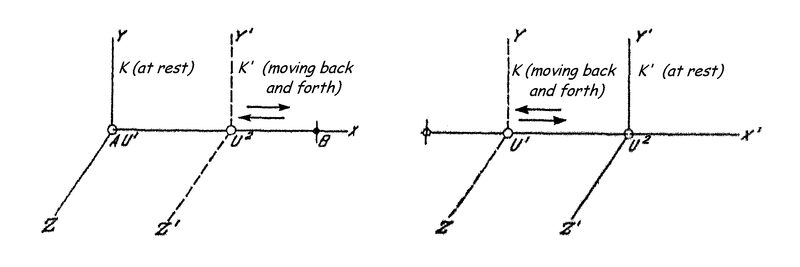
\includegraphics[width=5.0in]{figures/chapter1/exampleFig.png}}
    \caption{This figure comes from a paper written by Albert Einstein which I
    will cite here \cite{einstein1916foundation}.  \label{exampleFig}}
\end{figure}

You can create other directories in the ``figures'' directroy for the other
chapters in your disseration if you would like. This just helps keep things
organized.


\section{Dissertation/Thesis Objectives}

Its a good Idea to list the research objectives. Here is a way you can do it
in a list.
\begin{enumerate}
        \item Description of first objective corresponding to your first paper
            which is included as chapter 4. I can add labels to almost anything
            and reference them at other places in the text. Just make sure all
            your labels are unique throughout all of your included .tex
            documents \label{obj1}
        \item Description of next objective also corresponding to your first
            paper. \label{obj2}
        \item Description of your third objective which might correspond to your
            second paper presented in Chapter 5. \label{obj3}
\end{enumerate}

After this list I can reference objectives \ref{obj1} - \ref{obj3} like this.

\section{Dissertation/Thesis Structure}

Its also good to include a description of the structure of your dissertation/thesis
like what chapters include what info etc. You might do that here.

\chapter{Scientific Background}

This chapter can be used as your literature reveiw chapter and to include any
information on scientific theories that are particularly relevant to your
research. Here is an example of and equation.
%
\begin{equation}
    F_{es} = -\frac{1}{2} \int \epsilon(\mathbf{r}) \mathbf{E}^2(\mathbf{r}) dr
    \label{esfnrg}
\end{equation}
%
where $\epsilon(\mathbf{r})$ is the dielectric constant at position
$\mathbf{r}$ and $\mathbf{E}(\mathbf{r})$ is the electric field at the same
position. The equation can be referenced like this \ref{esfnrg}.

% \include{body/manuscript-style/citations}


% this is where the bibliography is included. Just add your bibtex citations
% to the citations.bib file and don't modify the code below unless you want to use
% a different citation style instead of "unsrtnat".
\singlespacing
\bibliographystyle{unsrtnat}
\bibliography{body/manuscript-style/citations}
\doublespacing


\end{document}
